
\documentclass[a4paper, norsk,  10pt]{article}
\usepackage[utf8]{inputenc}
\usepackage[norsk]{babel}
\usepackage[T1]{fontenc}
\usepackage{graphicx}
\usepackage{multirow}
\usepackage{varwidth}
\usepackage{amsmath}
\usepackage{algpseudocode}

\begin{document}

\title{Algoritmer og datastrukturer\\TDT4120\\Pensumoversikt}
\author{Håkon Ødegård Løvdal}
\date{Sist endret: \today}
\maketitle
\thispagestyle{empty}

\newpage

\section{Intro}

Dette dokumentet er skrevet for min egen del, i desperasjon for å tilegne meg pensum i TDT4120 høsten 2013. All informasjon er hentet fra Cormen og tilfeldige skumle steder på internett. All bruk og lesing skjer på eget ansvar. Du får ignorere eventuelle skrivefeil da det er raskt skrevet, uten korrekturlesning. Tex-fila er tilgjengelig på GitHub og OnlineWikien, så du er velkommen til å endre og modifisere som du selv vil! 

\section{Begreper}

\begin{center}
\begin{tabular}{|l|l|} 
\hline
\multirow{2}{*}{Algoritme} & En veldefinert prosedyre, som tar en verdi\\
	 & eller mengde verdier som input, og produserer\\
	& en verdi, eller mengde med verdier som output.\\
	& Det er en sekvens som transformerer input til output.\\ \hline 
	Problem			& Et problem er en relasjon mellom input og output. \\ \hline
	Probleminstans		& En probleminstans er en bestemt input. \\ \hline
	Iterasjon 		& En gjennomkjøring av en gjenntatt handling\\ \hline
	Asymtpoisk notasjon	& Notasjon hvor man kun tar vare på største ledd\\ \hline
\multirow{2}{*}{In-Place} & En algoritme er in-place når den operer på input dataen \\
	& uten å måtte lage feks nye array for å løse problemet.  \\ \hline
\multirow{2}{*}{Stabil} & At en algoritme er stabil vil si at hvis du sorterer en liste\\ 
	&med tall, vil alltid tallet i forekomsten som var først i den opprinnelige\\
	&listen komme først i den sorterte listen. \\ \hline
\end{tabular}
\end{center}

\section{Asymptotisk notasjon}

\begin{center}
\begin{tabular}{|l|l|l|}
    \hline
    Navn & Notasjon & Kjøretid \\ \hline
    Store-O & $O(n)$ & $\le n$ \\ \hline
    Theta & $\Theta(n)$ & $= n$ \\ \hline
    Store-Omega & $\Omega(n)$ & $\ge n$ \\ \hline
\end{tabular}
\end{center}

\subsection{Kompleksitetsklasser}

Grovinndeling i stigende rekkefølge:

\begin{enumerate}
\item Konstant: $1$
\item Polylogaritmisk: ${{(\log_{b}n})^{k}}$
\item Polynomisk: $n^k$
\item Eksponentiell: ${2^{n}}$
\item Faktoriell: $n!$
\item Alt som er enda verre, f.eks. $n^n$
\end{enumerate}

\subsection{Pseudopolynomialitet}

Gitt en algoritme som tar tallet $n$ som input og har kjøretid $O(n)$ – hvilken kompleksitetsklasse er dette? $n$ betegner her ikke størrelsen på input, men er selv en del av inputen. Det vil si at størrelsen til $n =$ antall bits som kreves $= \lg(n)$. 

\begin{center}
$n = {2^{\lg(n)}} = 2w \Rightarrow$ NB: Eksponentiell kjøretid! \
\end{center}

Dukker ofte opp som lureoppgave på eksamen!

\section{Kjøretider på pensumalgoritmer}

\begin{center}
\begin{table}[h]
\scalebox{0.8}{
\begin{tabular}{|l|l|l|l|l|}
\hline
\multirow{2}{*}{\textbf{Problem}}   & \multirow{2}{*}{\textbf{Algoritme}} & \multicolumn{3}{|c|}{\textbf{Kjøretid}} \\ \cline{3-5} 
                           &                            & \textbf{BC}      & \textbf{AC}            & \textbf{WC}  \\ \hline
\multirow{8}{*}{Sortering} & Insertion Sort             & $\Theta(n)$    & $\Theta(n^2)$   & $\Theta(n^2)$   \\ \cline{2-5} 
                           & Bubble Sort             &  $\Theta(n)$       &    $\Theta(n^2)$         &  $\Theta(n^2)$      \\ \cline{2-5} 
                           & Merge Sort                 &   $\Theta(n \lg(n))$     & $\Theta(n \lg(n))$  &    $O(n \lg(n))$    \\ \cline{2-5} 
                           & Heap Sort                  &    $O(n \lg(n))     &   $O(n \lg(n)) $         &  $O(n \lg(n))      \\  \cline{2-5} 
			& Quick Sort 		&	$\Theta(n \lg(n))	& $O(n \lg(n))$ 	&  $\Theta({n^{2}})$ \\  \cline{2-5} 
			& Counting Sort 	&	-	& $\Theta(n)$	& $\Theta(k + n)$ hvis $k = O(n)$ \\  \cline{2-5} 
			& Radix Sort 	& -	& $\Theta(d(n + k))$	& - \\  \cline{2-5} 
			& Bucket Sort & -	& $\Theta(n)$	& - \\ \cline{2-5} 
			\hline
\multirow{6}{*}{Grafer/Trær} & Toplogisk sortering & - & $\Theta(|V| + |E|)$ &- \\ \cline{2-5}
			& DFS & -& $\Theta(|V| + |E|)$ &- \\ \cline{2-5} 
			& BFS &- & $O(|V| + |E|)$ &- \\ \cline{2-5} 
			& Prim & $O(E \lg(V)$ & $\Theta(E \lg(V))$ &- \\ \cline{2-5} 
			& Kruskal & $O(E \lg(V)$ & $\Theta(E \lg(V))$ & -\\ \cline{2-5} 
			& Binærsøk & $O(\lg n)$ & - &  $O(\lg n)$  \\ \cline{2-5}
			\hline
\multirow{4}{*}{Korteste vei} & Bellman-Ford & -  & $O(|V| \times |E|)$ & -\\ \cline{2-5}
			& Dijkstra & $O(|E| \lg (|V|)$ (bin-heap) & $O({|V|^{2}})$ (array) &-  \\ \cline{2-5} 
			& DAG-Shortest Path &- & $\Theta(|V| + |E|)$ &- \\ \cline{2-5}
			& Floyd-Warshall &- & $\Theta({|V|^{3}})$  &- \\ \cline{2-5} 
			\hline
\multirow{2}{*}{Flyt} & Ford-Fulkerson &- & $O(E|f^*|)$ & ${f^{*}} = $ maks flyt i G \\ \cline{2-5}
			& Edmonds-Karp &- & $O(VE^2)$ &- \\ \cline{2-5}
			\hline
\multirow{1}{*}{Grådig} & Huffmann & $O(n \lg(n))$ &- & -\\ \cline{2-5}
			\hline
\end{tabular}}
\end{table}
\end{center}

\section{Rekurensanalyse}

\subsection{Masterteoremet}

Masterteoremet er en form for ``kokebok''-metode for å løse rekurenser. Man kan som regel løse de fleste rekurrenser av typen: 

\begin{center}
$T(n) = aT(\frac{n}{b}) + f(n)$
\end{center}
\noindent hvor $a \ge 1$ og $b > 1$. $f(n)$ må også være asymptotisk positiv. \\ \hfill

\begin{description}
\item[Case 1:] $f(n) = O(n^{\log_{b}a - \varepsilon})$ , for en $\varepsilon > 0$ \\ $\Rightarrow T(n) = \Theta(n^{\log_{b}a})$ 
\item[Case 2:] $f(n) = \Theta(n^{\log_{b}a})$  \\  $\Rightarrow T(n) = \Theta(n^{\log_{b}a} \log(n))$ 
\item[Case 3:] $f(n) = \Omega(n^{\log_{b}a + \varepsilon})$, for en $\varepsilon > 0$ og $af(\frac{n}{b}) \leq cf(n)$, hvor $c < 1$ \\  $\Rightarrow T(n) = \Theta(f(n))$
\end{description}

\subsubsection{Bruk av masterteoremet}

Gitt et problem i hver ``case'':

\begin{enumerate}
\item $T(n)=4T(\frac{n}{2})+n$
\item $T(n)=4T(\frac{n}{2})+{n^{2}}$
\item $T(n)=4T(\frac{n}{2})+{n^{3}}$
\end{enumerate} 

\noindent I disse problemene er $a=4, b=2$ og $f(n)$ henholdsvis $n, {n^{2}}, {n^{3}}$. I alle disse tilfellene vil vi sammenligne $f(n)$ med ${n{^{\log_{b}a}}$ $\Rightarrow ${n{^{\log_{2}4}} \Rightarrow {n^{2}}$.

\begin{description}
\item[Case 1:] $f(n)=n=O({n^{2-\varepsilon}})$ for $\varepsilon=0.5$. Altså $T(n)=\Theta({n^{{\log_{b}a}}})=\Theta({n^{2}})$
\item[Case 2:] $f(n)={n^{2}}=\Theta({n^{2}})$. Altså $T(n)=\Theta({n^{{\log_{b}a}}}\log n)=\Theta({n^{2}} \log n)$
\item[Case 3:] $f(n)={n^{3}}=\Omega({n^{2+\varepsilon}})$ for $\varepsilon=0.5$ og $af(\frac{n}{b}) \leq cf(n)$, feks. $4{(\frac{n}{2})^{3}} = \frac{n^{3}}{2} \leq {cn^{3}}$ for $c={\frac{1}{2}$. Altså $T(n)=\Theta(f(n))=\Theta({n^{3}})$
\end{description}

\subsection{Eksempel på rekursens fra desember 2007}

\begin{center}
\begin{table}[h]
\scalebox{0.8}{
\begin{tabular}{|l|l|l|l|l|}
\hline
Rekursive kall & Størrelse, delproblem & Arbeid i hvert kall & Rekurrens & Kjøretid \\ \hline
Ett & Redusert med 1 & Konstant & $T(n)=T(n-1) + \Theta(1)$ & $\Theta(n)$  \\ \hline
Ett & Halvert & Konstant & $T(n)=T(\frac{n}{2}) + \Theta(1)$ & $\Theta(\lg n)$ \\ \hline
Ett & Redusert med 1 & Lineært & $T(n)=T(n-1) + \Theta(n)$ & $\Theta({n^{2}})$ \\ \hline
Ett & Halvert & Lineært & $T(n)=T(\frac{n}{2}) + \Theta(n)$ & $\Theta(n)$ \\ \hline
To & Redusert med 1 & Konstant & $T(n)=2T(n-1) + \Theta(1)$ & $\Theta({2^{n}})$ \\ \hline
To & Halvert & Konstant & $T(n)=2T(\frac{n}{2}) + \Theta(1)$ & $\Theta(n)$ \\ \hline
To & Redusert med 1 & Lineært & $T(n)=2T(n-1) + \Theta(n)$ & $\Theta({2^{n}})$ \\ \hline
To & Halvert & Lineært & $T(n)=2T(\frac{n}{2}) + \Theta(n)$ & $\Theta(n \lg n)$\\ \hline
\end{tabular}}
\end{table}
\end{center}

\noindent Merk at siste rekursen er løst med masterteoremet, mens de andre er løst uten. 

\begin{center}
tid $= \#$ subproblemer $\times$ tid per subproblem
\end{center}

\section{Datastrukturer}

\begin{center}
\begin{tabular}{|l|l|l|l|}
    \hline
                                & Lenket liste       & Array    & Dynamisk Array \\ \hline
    Indeksering             & $\Theta(n)$          & $\Theta(1)$ & $\Theta(1)$      \\ \hline
    Ins/del front & $\Theta(1)$          & -        & $\Theta(n)$      \\ \hline
    Ins/del bakerst       & $\Theta(n)$          & -        & $\Theta(1)$      \\ \hline
    Ins/del midten    & Søk + $\Theta(1)$ & -        & $\Theta(n)$      \\ \hline
    Ubrukt plass         & $\Theta(n)$          & $0$        & $\Theta(n)$      \\ \hline
\end{tabular}
\end{center}

\subsection{Stack}

Stack er en \textit{LIFO}, ``Last In, First Out''-datastruktur. Stack implementeres oftest med et array, eller en lenket liste. En stack har egenskapene \textit{INSERT, PUSH} og \textit{POP (DELETE)}. 

\begin{figure}[hbt]
    \begin{center}
        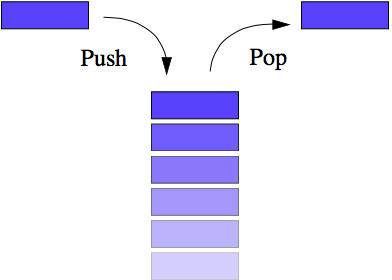
\includegraphics[width=5cm] {stack.png}
        \caption{Enkel illustrasjon av en stack}
    \end{center}
\end{figure}

\subsection{Kø/Queue}

Kø er en \textit{FIFO}, ``Fist In, First Out''-datastruktur. En kø implementeres som oftest som et array (gjerne et dynamisk array, likt Java sin \textit{ArrayList}. En kø har egenskapene \textit{ENQUEUE} og \textit{DEQUEUE}.

\begin{figure}[hbt]
    \begin{center}
        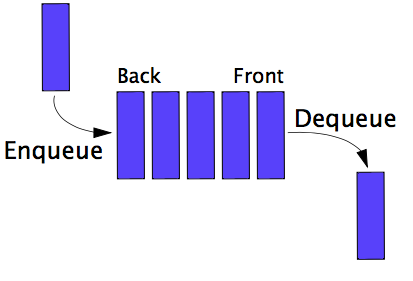
\includegraphics[width=5cm] {ko.png}
        \caption{Enkel illustrasjon av en kø}
    \end{center}
\end{figure}

\subsection{Lenket-liste}

En lenket liste er en datastruktur hvor objektene er ordnet lineært. Hvert objekt har helst to peker-variabler, \textit{next} og \textit{prev}. Har den begge disse peker-variablene er det en dobbelt lenket liste. Ved kun en peker (\textit{next}) er det en enkelt-lenket liste. 

\begin{figure}[hbt]
    \begin{center}
        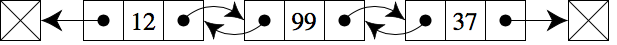
\includegraphics[width=7cm] {linked.png}
        \caption{Enkel illustrasjon av en dobbelt lenket liste}
    \end{center}
\end{figure}

\subsection{Binært søketre}

Et binært søketre er et tre som tilfredstiller \textit{binært-søketre-egenskapen}. 

\begin{center}
\begin{tabular}{|l|l|l|}
    \hline
    Operasjon & Average & Worst \\ \hline
    Plass (bit)     & $O(\log n)$       & $O(n)$     \\ \hline
    Søk    & $O(\log n)$       & $O(n)$     \\ \hline
    Sett inn    & $O(\log n)$       & $O(n)$     \\ \hline
    Slett    & $O(\log n)$       & $O(n)$     \\ \hline
\end{tabular}
\end{center}

\subsubsection{Binært-søketre-egenskapen}

La $x$ være en gitt node i søketreet. Hvis $y$ er en node i det venstre subtreet til $x$ må $y$ sin verdi være mindre eller lik ($\leq$) $x$ sin verdi. \\
\noindent Tilsvarende for høyre subtre. Her må $y$ sin verdi være større enn eller lik ($\geq$) $x$ sin verdi.


\begin{figure}[hbt]
    \begin{center}
        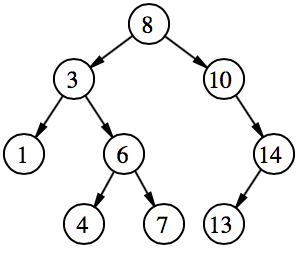
\includegraphics[width=5cm] {binarytree.png}
        \caption{Et binært søketre}
    \end{center}
\end{figure}

\subsubsection{Traversering av binæretrær}

Vi benytter oss av tre måter å traversere et binært tre på, disse er:

\begin{description}
\item[Preorder] Her printer man ut nodens verdi før dens barn, venstre og deretter høyre.
\item[Inorder] Her printer man venstre barn, noden, og deretter høyre barn (om ikke det er noe venstre barn, print noden før høyre barn)
\item[Postorder] Her printer man nodens verdi etter man har printet venstre og høyre barn
\end{description}

\begin{figure}[hbt]
    \begin{center}
        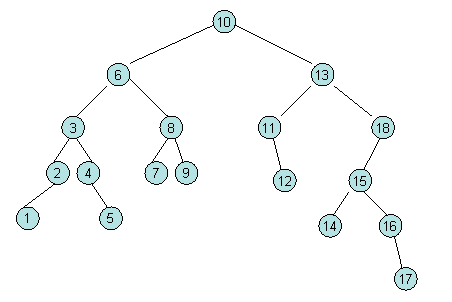
\includegraphics[width=7cm] {bintrav.png}
        \caption{Enkelt binærtre for traverseringseksempel}
    \end{center}
\end{figure}

\noindent Et eksempel fra figur 5:
\begin{description}
\item[Preorder] 10, 6, 3, 2, 1, 4, 5, 8, 7, 9, 13, 11, 12, 18, 15, 14, 16, 17
\item[Inorder] 1, 2, 3, 4, 5, 6, 7, 8, 9, 10, 11, 12, 13, 14, 15, 16, 17, 18
\item[Postorder] 1, 2, 5, 4, 3, 7, 9, 8, 6, 12, 11, 14, 17, 16, 15, 18, 13, 10
\end{description}

\subsection{Hasing}

Hashing er en effektiv måte å lagre $(key, value)$-pairs. Istedenfor at indeksen er nøkkelen, er heller indeksen basert på nøkkelen med en hashfunksjon. 

\begin{center}
\begin{tabular}{|l|l|l|}
        \hline
        Operasjon      & WC & BC \\ \hline
        Søke  & $O(1) & $O(n)$ \\ \hline
        Sett inn  & $O(1)& $O(n)$ \\ \hline
        Slette  & $O(1)& $O(n)$ \\ \hline
        Plass  & $O(n) &$O(n)$ \\ \hline
\end{tabular} \\
\textit{Kommentar: Usortert array}
\end{center}

\subsubsection{Direct-address tables}

Fungerer best/optimalt når mengen mulige nøkler ($n$) er forholdsvis lav. Ved å lage en tabell med $n$ felter, kan hver indeks representere en nøkkel. 

\subsubsection{Hash-tables}

En mer effektiv måte å lage en slik tabell på. Man har en mindre tabell enn antall elementer. Hvert felt har derimot en egen nøkkel. Disse nøkklene blir generert av hashfunksjonen, $h(k)$. På grunn av at tabellen er mindre enn antall elementer kan kollisjoner oppstå (flere nøkler, gir samme hashverdi). Vi har flere metoder for å løse kollisjoner. Her brukes feks. \textbf{\textit{chaining}}.

\subsection{Heap}

En heap er en spesiell trestruktur, som tilfredstiller heap-egenskapen. 
Det finnes ingen regler for hvordan søsken er ordnet i heapen. 
En heap er ofte implementert med et array. Det er viktig å legge merge til at første indeks skal være tom. Det vil si at i et 0-indeksert array vil plass 0 være tom, mens første node står på indeks 1.

\begin{center}
\begin{tabular}{|l|l|}
        \hline
        Operasjon      & Tidskompleksitet \\ \hline
        Finn min/max   & $\Theta(1)$ \\ \hline
        Slett min/max & $\Theta(\log n)$ \\ \hline
        Sett inn         & $\Theta(\log n)$               \\ \hline
        Omstrukturere heap   & $\Theta(\log n)$              \\ \hline
        Merge          & $\Theta(n)$ \\ \hline
\end{tabular}\\
\textit{Kommentar: Min/max avhenger om det er min/max heap}
\end{center}

\begin{figure}[hbt]
    \begin{center}
        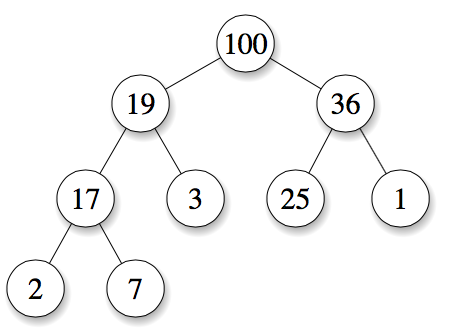
\includegraphics[width=5cm] {heap.png}
        \caption{En liten max-heap}
    \end{center}
\end{figure}

\subsubsection{Heap-egenskapen}

I en heap må hele treet være fullstendig fylt ut, bortsett fra muligens det laveste nivået, som fylles ut fra venstre.

\begin{itemize}
\item Rotnode: $i=1$ 
\item Foreldrenode(i): $i/2$ 
\item Høyre-barn: ($2i + 1$), Venstre-barn: ($2i$) 
\end{itemize}

\noindent \textbf{Max-Heap:} \\ \hfill

\noindent For hver node $i$, bortsett fra rot-noden, må verdien til barnenode være mindre eller lik foreldrenoden. $A[PARENT(i)] \geq A[i]$ \\ \hfill

\noindent \textbf{Min-Heap:} \\ \hfill

\noindent For hver node $i$, bortsett fra rot-noden, må verdien til en barnenode være større eller lik foreldre noden. $A[PARENT(i)] \leq A[i]$

\section{Sorteringsalgoritmer}

\subsection{Insertion Sort}

Insertion Sort er en enkel sorteringsalgoritme. Den tar de to første elementene og plasserer i forhold til hverandre. Deretter plasserer den det neste i forhold til de to forrige, osv. Veldig effektiv å bruke på små mengder. Kan feks. brukes i slutten på en Quick Sort algoritme. \\

\begin{algorithmic}
\For {$j=0$ to $A.length$}
	\State $key = A[j]$ 
	\State $i = j - 1$ 
	\While {$i > 0$ and $A[i] > key$}
		\State $A[i + 1] = A[i]$ 
		\State $i = i - 1$ 
	\EndWhile
	\State $A[i] + 1 = key$ 
\EndFor
\end{algorithmic}

\subsection{Bubble Sort}

Bubble Sort testet to og to naboelementer. Dersom den første er større bytter de plass. Effektiv på små datamengder. \\

\begin{algorithmic}
\For {$i=0$ to $A.length - 1$}
	\For {$j=A.length$ downto $i + 1$}
		\If {$A[j] < A[j -1]$}
			\State exchange $A[j]$ with $A[j-1]$
		\EndIf
	\EndFor
\EndFor
\end{algorithmic}

\subsection{Merge Sort}

Merge Sort er en ``splitt-og-hersk''-algoritme. Merge Sort er effektiv. Deler opp problemet i stadig mindre biter, og når bitene er små nok flettes de sammen i sortert rekkefølge. \\

\begin{algorithmic}
 \Function{MERGE-SORT}{$A, p, r$} 
	\If {$p < r$}
		\State $q = \lfloor(p + r) / 2 \rfloor $ 
		\State \Call{MERGE-SORT}{$A, p, q$} 
		\State \Call{MERGE-SORT}{$A, q + 1, r$}
		\State \Call{MERGE}{$A, p, q, r$} 
	 \EndIf
\EndFunction
\State 

\Function{MERGE}{A, p, q, r}
\State ${n_{1}}=q-pr+1$
\State ${n_{2}}=r-q$
\State let $L[1 \dots {n_{1}} + 1]$ and $R[1 \dots {n_{2}+1}$ be new arrays
\For {$i=1$ to ${n_{1}}$}
	\State $L[i] = A[p + i -1]$
\EndFor
\For {$j=1$ to ${n_{2}}$}
	\State $R[j] = A[q + j]$
\EndFor
\State $L[{n_{1}}] + 1] = \infty$
\State $r[{n_{2}}] + 1] = \infty$
\State $i = 1$
\State $j = 1$
\For {$k=p$ to $r$}
	\If {$L[i] \leq R[j]$}
		\State $A[k] = L[i]$
		\State $i = i + 1$
	\Else 
		\If  {$A[k] = R[j]$}
			\State $j = j + 1$
		\EndIf	
	\EndIf
\EndFor
\EndFunction
\end{algorithmic}

\subsection{Heap Sort}

Heapsort benytter seg av en heap som datastruktur. Lager en heap av alle elementene sik at hver node sine barn er mindre enn den selv. Det øverste elementet er alltid det største. Deretter plukkes det øverste elemtentet ut, for så å sortere heapen igjen, og ta ut det øverste elementet igjen. Fortsetter til heapen er tom.  \\

\begin{algorithmic}
\State \Call{BUILDMAXHEAP}{$A$} 
\For {$i = A.length$ downto $2$}
	\State exchange $A[1]$ with $A[i]$
	\State $A.heapSize$ = $A.heapSize -1$
	\State \Call{MAX-HEAPIFY}{$A, 1$} 
\EndFor
\end{algorithmic}

\subsection{Quick Sort}

Quick Sort er enda en ``split-og-hersk''-algoritme. Man starter gjerne Quick Sort ved å randomisere lista. Den starter med å velge et pivotelement. Den deler deretter lista i to partisjoner: en med elementene som er mindre eller lik pivoten, og en med elementene som er større en pivot. Deretter kaller den seg selv rekursivt på de to partisjonene. Deretter fletter man sammen de to partisjonene.  \\

\begin{algorithmic}
\Function{QUICKSORT}{$A, p, r$}
\If {$p < r$}
	\State $q$ = \Call{PARTITION}{$A, p , r$}
	\State \Call{QUICKSORT}{$A, p, q -1$}
	\State \Call{QUICKSORT}{$A. q + 1, r$}
\EndIf
\EndFunction \\

\Function{PARTITION}{$A, p, r$}
	\State $x = A[r]$
	\State $i = p - 1$
	\For {$j = p$ to $r -1$}
		\If {$A[j] \leq x$}
			\State $i = i + 1$
			\State exchange $A[i]$ with $A[j]$
		\EndIf
	\EndFor
\State exchange $A[i + 1]$ with $A[j]$
\State \Return{$i + 1$}
\EndFunction
\end{algorithmic}

\subsection{Counting Sort}

Counting Sort tar et heltall $N$ mellom $0$ og $k$. Lager en liste med vardier fra $0$ til $k$ og setter inn tallene på sin plass i lista. Fungerer best når verdiene på tallene som sorteres ligger tett etterhverandre og $k$ ikke er for høy. \\

\begin{algorithmic}
\Function{COUNTINGSORT}{$A, B, k$}
\State let $C[0 \dots k]$ be a new array
\For {$i=0$ to $k$}
\State $C[i]=0$
\EndFor
\For {$j=1$ to $A.length$}
\State $C[A[j]] = C[A[j]] + 1$
\EndFor
\For {$i=0$ to $k$}
\State $C[i] = C[i] + C[i -1]$
\EndFor
\For {$j=A.length$ downto $1$}
\State $B[C[A[j]]] = A[j]$
\State $C[A[j]] = C[A[j]] - 1$
\EndFor
\EndFunction
\end{algorithmic}

\subsection{Radix Sort}

Radix Sort sorterer tall i et gitt tallsystem (her titallsystemet) etter minst signifikante siffer. \\

\begin{algorithmic}
\Function{RADIXSORT}{$A, d$}
\For {$i = 1$ to $d$}
	\State Bruk \textit{Stable Sort} til å sortere array $A$
\EndFor
\EndFunction 
\end{algorithmic}

\subsection{Bucket Sort}

Veldig lik Counting Sort, men bruker såkalte ``bøtter'' man putter tallene i. For eksempel $[5, 6)$ betur at verdier større eller lik 5, men mindre enn 4 skal i bøtta. \\

\begin{algorithmic}
\Function{BUCKETSORT}{$A$}
\State $n = A.length$
\State la $B[0 \dots n - 1]$ være et nytt array
\For {$i = 0 $ to $n - 1$}
	\State Gjør $B[i]$ til en tom liste
\EndFor
\For {$i = 1$ to $n$}
	\State Sett inn $A[i]$ i lista $B[ \lfloor nA[i] \rfloor ]$
\EndFor
\For {$i = 0$ to $n - 1$}
	\State Sorter lista $B[i]$ med \Call{InsertionSort}{B[i]} 
\EndFor
\State Konkatiner listene $B[0], B[1], \dots , B[n - 1]$ i rekkefølge
\EndFunction 
\end{algorithmic}

\section{Grafer/Trær}

\subsection{Dybde først-søk}

DFS implementeres med en stack. 
DFS utforsker grafen i dybden. Den fyller stacken med noder den støter på. Kan man ikke går videre vil den ``backtrace'' til forrige node, og se etter en mulig vei videre. Hvis stacken er tom, sjekker man om alle noder er besøkt. Hvis ikke, starter man på nytt fra ubesøkte noder. 


\begin{algorithmic}
\Function{DFS}{$G, v$} \Comment v er startnode
	\State initaliser en tom stack, $S$
	\For {each vertex $u$ in G}
	\State set $visited[u] \rightarrow false$
	\EndFor 
	\State $S.push(v)$
	\While{$S.notEmpty()$}
		\State $u = S.pop()$
		\For {all $w$ adjacent to $u$}
			\If {not $visited[w]$}
				\State $visited[w] \rightarrow true$
				\State $S.push(w)$
			\EndIf
		\EndFor
	\EndWhile
\EndFunction
\end{algorithmic}

\subsection{Bredde først-søk}

BFS implementeres med en kø.
BFS utforsker grafen i bredden. Man starter på foreldrenoden og legger inn alle dens barn i køen. Når alle naboer til node $x$ er oppdaget, fjernes den fra køen og man tar den neste noden i køen, og legger alle dens barn inn i køen. Når køen er tom, sjekker man ikke videre om det er ubesøkte noder. 

\begin{algorithmic}
\Function{BFS}{$G, v$} \Comment v er startnode 
	\State lag en kø $Q$
	\State legg $v$ inn i $Q$
	\While {$Q.notEmpty()$}
		\State $v = Q.dequeue()$
		\For {each edge $e$ adjacent to $v$}
			\If {$e$ not marked}
				\State mark $w$
				\State $Q.enqueue(e)$
			\EndIf
		\EndFor
	\EndWhile
\EndFunction

\subsection{Topologisk sortering}

Topologisk sortering bruker en DAG til å finne en rekkefølge igjennom alle elementene i grafen. Det tillates ikke sykler. Man begynner i noden som ikke har noen kanter inn til seg. 

\begin{algorithmic}
\Function{TOPOLOGICALSORT}{$G$}
\State \Call{DFS}{$G$} to compute finish times $v.f$ for each vertex $v$.
\State as each vertex is finished, insert it onto the end of the list
\State \Return{the list of verticies}
\EndFunction
\end{algorithmic}

\subsection{Minimale spenntrær}

\subsubsection{Prims algoritmer}

Prims algoritme velger en tilfeldig node, og legger alle kantene inn i en prioritetskø etter vekt. Velger den billigste kanten og legger den til i treet.  Det vil si at den legger til den billigste kanten som er mulig å legge til fra treet den bygger. \\ \hfill

\begin{algoritmic}
\Function {PRIM}{G, w, r}
\For {each $u \in G.V$}
	\State $u.key = \infty$
	\State $u.\pi = NIL$
\EndFor
\State $r.key = 0$
\State $Q = G.V$
\While {$Q \neq \emptyset$}
	\State $u = \Call{EXTRACT-MIN}{Q}$
	\For {each $v \in G.Adj[u]$}
		\If {$v \in Q$ and $w(u, v) < v.key$}
			\State $v.\pi = u$
			\State $v.key = w(u, v)$
		\EndIf
	\EndFor
\EndWhile
\EndFunction
\end{algoritmic}

\subsubsection{Kruskals algoritme}

Kruskals algoritme sorterer alle kanter etter kostnaden og velger den billigste tilgjengelige kanten , og legger til denne med noder i treet. Dette kun hvis den ikke allerede er brukt og vil danne en sykel. Fortsetter til det ikke finnes kanter som kan legges til i treet.  \\ \hfill

\begin{algoritmic}
\Function {KRUSKAL}{G, w}
\State $A = \emptyset$
\For {each vertex $v \in G.V$}
	\State \Call{MAKE-SET}{$v$}
\EndFor
\State sort edges of $G.E$ into nondecreasing order by weight $w$
\For {each edge $(u,v) \in G.E$, taken in nondecreasing order by weight}
	\If {\Call{FIND-SET}{$u$} $\neq$ \Call{FIND-SET}{$v$}}
		\State $A = A \cup \{ (u,v) \}$
		\State \Call{UNION}{u,v} 
	\EndIf  
\EndFor
\State \Return{$A$}


\EndFunction
\end{algoritmic}

\section{Korteste-vei-algoritmer}

Det er flere gode algoritmer for å løse korteste-vei problemet. \\

\begin{algoritmic}
\Function{RELAX}{u, v, w}
	\If {$v.d > u.d + w(u, v)$}
		\State $v.d = u.d + w(u, v)$
		\State $v.\pi = u$ 
		\State Cormen bruker $\pi$ til å representere foreldrenode.
	\EndIf
\end{algoritmic}

\subsection{Bellman-Ford} 

Bellman-Ford er en korteste vei, en-til-alle algoritme. Den tillater negative kanter. Returnerer $false$ dersom det finnes en negativ sykel i grafen. Går igjennom alle kantene og bruker $RELAX$ på hver av dem $|V|-1$ ganger. Deretter sjekker den etter negative sykler ved å sjekke om veien fra startnoden til node $w$ via node $v$ blir mindre enn den vi fant under søket. \\ \hfill

\begin{algoritmic}
\Function{BELLMANN-FORD}{$G, w, s$}
\State \Call{INITIALIZE-SINGLE-SOURCE}{$G, s$}
\For {$i = 1$ to $|G.V| - 1$}
	\For {each edge $(u, v) \in G.E$}
		\State \Call{RELAX}{$u, v, w$}
	\EndFor
\EndFor
\For {each edge $(u, v) \in G.E$}
	\If {$v.d > u.d + w(u, v)$}
		\State \Return $false$
	\EndIf
\EndFor
\State \Return $true$
\EndFunction

\end{algoritmic}

\subsection{Dijkstra}

Dijkstra er en korteste vei, en-til-alle algoritme. Tillater ikke negative kanter. Den velger noder en etter en fra hvor nærme de er startnoden. Dijkstra er en grådig algoritme. \\ \hfill

\begin{algoritmic}
\Function{DIJKSTRA}{$G, w, s$}
\State \Call{INITIALIZE-SINGLE-SOURCE}{$G, s$}
\State $S = \emptyset$
\State $Q = G.V$
\While {$Q \neq \emptyset$}
	\State $u = $ \Call{EXTRACT-MIN}{Q}
	\State $S = S \cup \{u\}$
	\For {each vertex $v \in G.Adj[u]$}
		\State \Call{RELAX}{u, v, w}
	\EndFor
\EndWhile
\EndFunction

\end{algoritmic}

\subsection{DAG-Shortest path}

DAG-Shortest-Path er en korteste vei, en-til-alle algoritme. Tillater ikke negative kanter, og kan selvfølgelig ikke ha sykler, da det er en DAG. Gjør topologisk sortering av DAGen og besøker hver node \textit{en} gang for å kjøre $RELAX$ på nodene foran. \\ \hfill

\begin{algoritmic}
\Function{DAG-SHORTEST-PATH}{G, w, s}
\State \Call{TOPOLOGICAL-SORT}{G}
\State \Call{INITIALIZE-SINGLE-SOURCE}{G, s}
\For {each vertex $u$, taken in topologically sorted order}
	\For {each vertex $v \in G.Adj[u]$}
		\State \Call{RELAX}{u, v, w}
	\EndFor
\EndFor
\EndFunction
\end{algoritmic}

\subsection{Floyd-Warshall}

Floyd-Warshall er en korteste vei, alle-til-alle algoritme. Den bruker DP. Lager en nabomatrise for alle noder og hvor det går kanter. Kostnaden mellom disse blir verdien av kanten. Er det ikke en direkte vei mellom to noder settes verdien til $\infty$. Deretter velges den en node $a$ og sjekker om veien fra $u$ til $v$ er kortere via $a$. Deretter finner den en ny node, og sjekker om det er kortere veier om man benytter seg av denne. Slik fortsetter den til den har besøkt alle noder.  \\ \hfill

\begin{algoritmic}
\Function{FLOYD-WARSHALL}{$W$}
\State ${D^{(0)} = W$
\For {$k = 1$ to $n$}
	\State let ${D^{(k)}$ be a $n$ x $n$ matrix
	\For {$i = 1$ to $n$}
		\For {$j = 1$ to $n$}
			\State ${D_{ij}^{(k)} = min(${D_{ij}^{(k-1)}, {D_{ik}^{(k-1)} + {D_{kj}^{(k-1)})$
		\EndFor
	\EndFor
\EndFor
\State \Return ${D^{(n)}$
\EndFunction

\end{algoritmic}

\section{Flyt-algoritmer}

\subsection{Ford-Fulkerson metoden}

Ford-Fulkerson metoden finner maksimal flyt i et flytnettverk. Hver iterasjon forsøker å finne en flytforøkende sti, og setter på all den flyten som er mulig. Deretter leter den etter en ny flytforøkende sti, og gjentar prosessen. Når det ikke er flere flytforøkende stier har man oppnåd maksimal flyt. Den benytter seg av DFS for å finne flytforøkende sti. 

\subsection{Edmonds-Karp Algoritmen}

Endret en bokstav på Ford-Fulkerson metoden. De benytter seg av BFS. Edmonds-Karp bruker Ford-Fulkerson og BFS til å finne flytforøkende stier. 

\subsection{Max Flow/Min Cut}

Minimum-snitt (min-cut) på et flytnettverk: det snittet som har lavest kapasitet av alle snitt. Det vil si \textit{min-cut} angir en flaskehals i flytnettverket. Det vil si at det ikke kan sendes mer flyt gjennom nettverket enn det vi kan sende gjennom flaskehalsen. Man kan da ikke finne noen flytforøkende sti over flaskehalsen. Det vil da være maksimal-flyt, \texit{max-flow}.

\begin{figure}[hbt]
    \begin{center}
        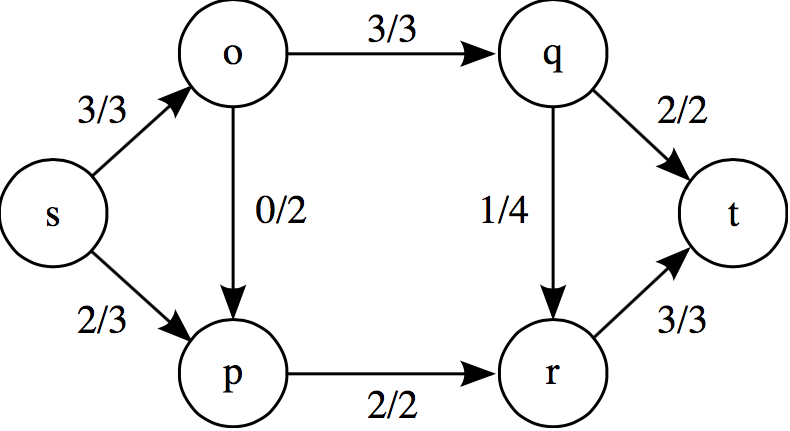
\includegraphics[width=5cm] {flow.png}
        \caption{Et lite flytnettverk}
    \end{center}
\end{figure}

\section{Grådighet}

En grådig algoritme er en algoritme som velger den beste lokale løsningen. Det vil si at den velger en lokalt optimalt løsning i håp om at den også skal være globalt optimal. 

\subsection{Huffmann}

Huffman-koding er en komprimeringsalgoritme. Den bruker et binærtre som baserer seg på frekvensen til bokstaver til å finne en prefikskode med ulik bitlengde for alle bokstavene. 

\begin{center}
\begin{figure}[hbt]
    \begin{center}
        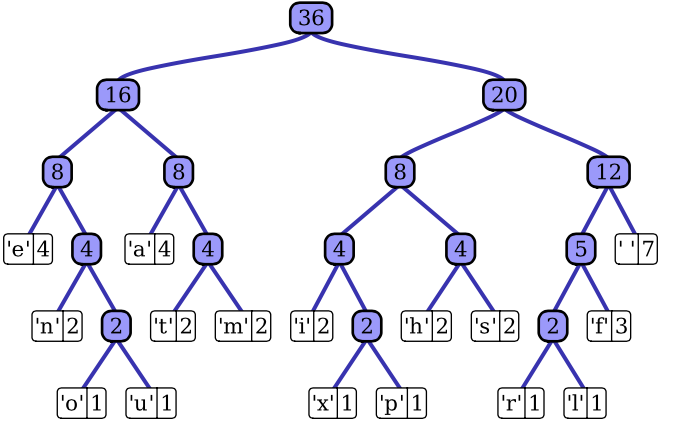
\includegraphics[width=8cm] {huff.png}
        \caption{Et lite Huffmanntre}
    \end{center}
\end{figure}
\end{center}

\section{Dynamisk Programmering}

DP $\approx$ rekursjon $+$ memoisering $\Rightarrow$ $tid/subproblemer =  \Theta(1)$ (teller ikke rekursjoner)

\subsubsection{Memoiserings DP-algoritme}

Memoisere betyr i hovedsak å huske og gjennbruke løsninger fra subproblemer for å løse problemet \\
\noindent $tid = \#subproblemer$ 

\noindent Et eksempel er en rekursiv fibonacci hvor man bruker en dictionary til å holde på tidligere utregnede subproblemer. 

\subsubsection{Bottom-Up DP-algoritme}

Veldig lik memoiserings algoritmen, men lagrer verdiene i en hashmap/dictionary og går fra 1 til $n$. Et eksempel er en implementasjon av $Fibonacci$ med $for-loop$ hvor man går fra 1 til $n$. For å spare plass kan man lagre kun de to siste elementene, da det er de som er interessante for å regne ut neste fibonacci-tall. 

\subsubsection{Fem enkle steg:}

\begin{enumerate}
\item definer subproblemene $(\#)$
\item gjett (del av løsning) $(\#)$
\item rekurens $(tid/subproblemer)$
\item \textit{rekursivt + memoisering} $\vee$ \textit{bottom-up}
\begin{enumerate}
	\item sjekk om den er asyklisk $\vee$ toplogisk sortert
	\item tid $= \#$ subproblemer $\times$ tid per subproblem
\end{enumerate}
\item løs det orginale problemet
\end{enumerate}

\section{NP-Komplette problemer}

\noindent NP $\Rightarrow$ Nondeterministic Polynomial \\
\noindent NPC $\Rightarrow$ NP-Complete\\
\noindent P $\Rightarrow$ Polynomial \\ \\

\noindent Et problem er NPC hvis det er et ``decisionproblem" og NP-Hard hvis det er  et ``opptimaliseringsproblem". \\ \\

\noindent \textbf{Sammenhengen mellom alle NP-problemer:} \\

$P \subseteq NP$ \\
$NPC \subseteq NP$ \\ \\

\noindent Hvis et problem $A \in NPC$, så vil også $A \in NP$. Dette er fordi $NP = P + NPC$. Hvis noe ikke er i P eller NPC, er det heller ikke i NP, fordi $P \cap NPC = \emptyset$. \\ \hfill
\begin{figure}[hbt]
    \begin{center}
        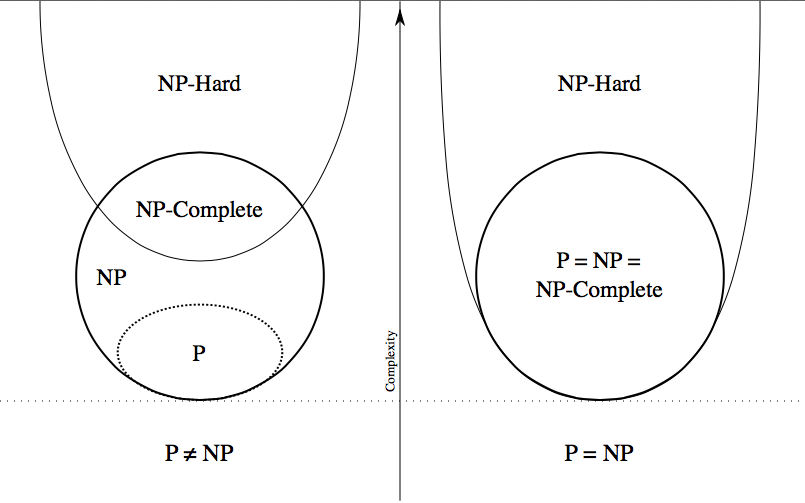
\includegraphics[width=7cm] {npc.png}
        \caption{Venndiagramet, med med $P \neq NP$ og $P = NP$}
    \end{center}
\end{figure}

\noindent Du vet at problem A er i NP og problem B er i NPC. Du vil vise at A også er i NPC. Da reduserer du fra B til A.\\ \hfill

\noindent Du står overfor de tre problemene A, B og C. Alle tre befinner seg i mengden NP. Du vet at A er i mengden P og at B er i mengden NPC. Anta at du skal bruke polynomiske reduksjoner mellom disse problemene til å vise $\dots$:

\begin{enumerate}
	\item $\dots$ at C er i P må $C \leq A$ (C reduseres til A)
	\item $\dots$ at C er i NPC må $B \leq C$ (B reduseres til C)
	\item $\dots$ hvis B kan reduseres til A er $P = NP$ (NB: ikke løst enda)
	\item Alle disse reduksjonene skjer i polynomisk tid
\end{enumerate}

\noindent To ikke helt legitime, men greie huskeregeler: 
\begin{center}
\textit{reduser fra litt til mer // fra litt \dots $\leq$ \dots til mer\\ }
\textit{reduser nedover: NPC $\rightarrow$ (NP) $\rightarrow$ P (forsiktig med denne)\\ \hfill}
\end{center}

\begin{figure}[hbt]
    \begin{center}
        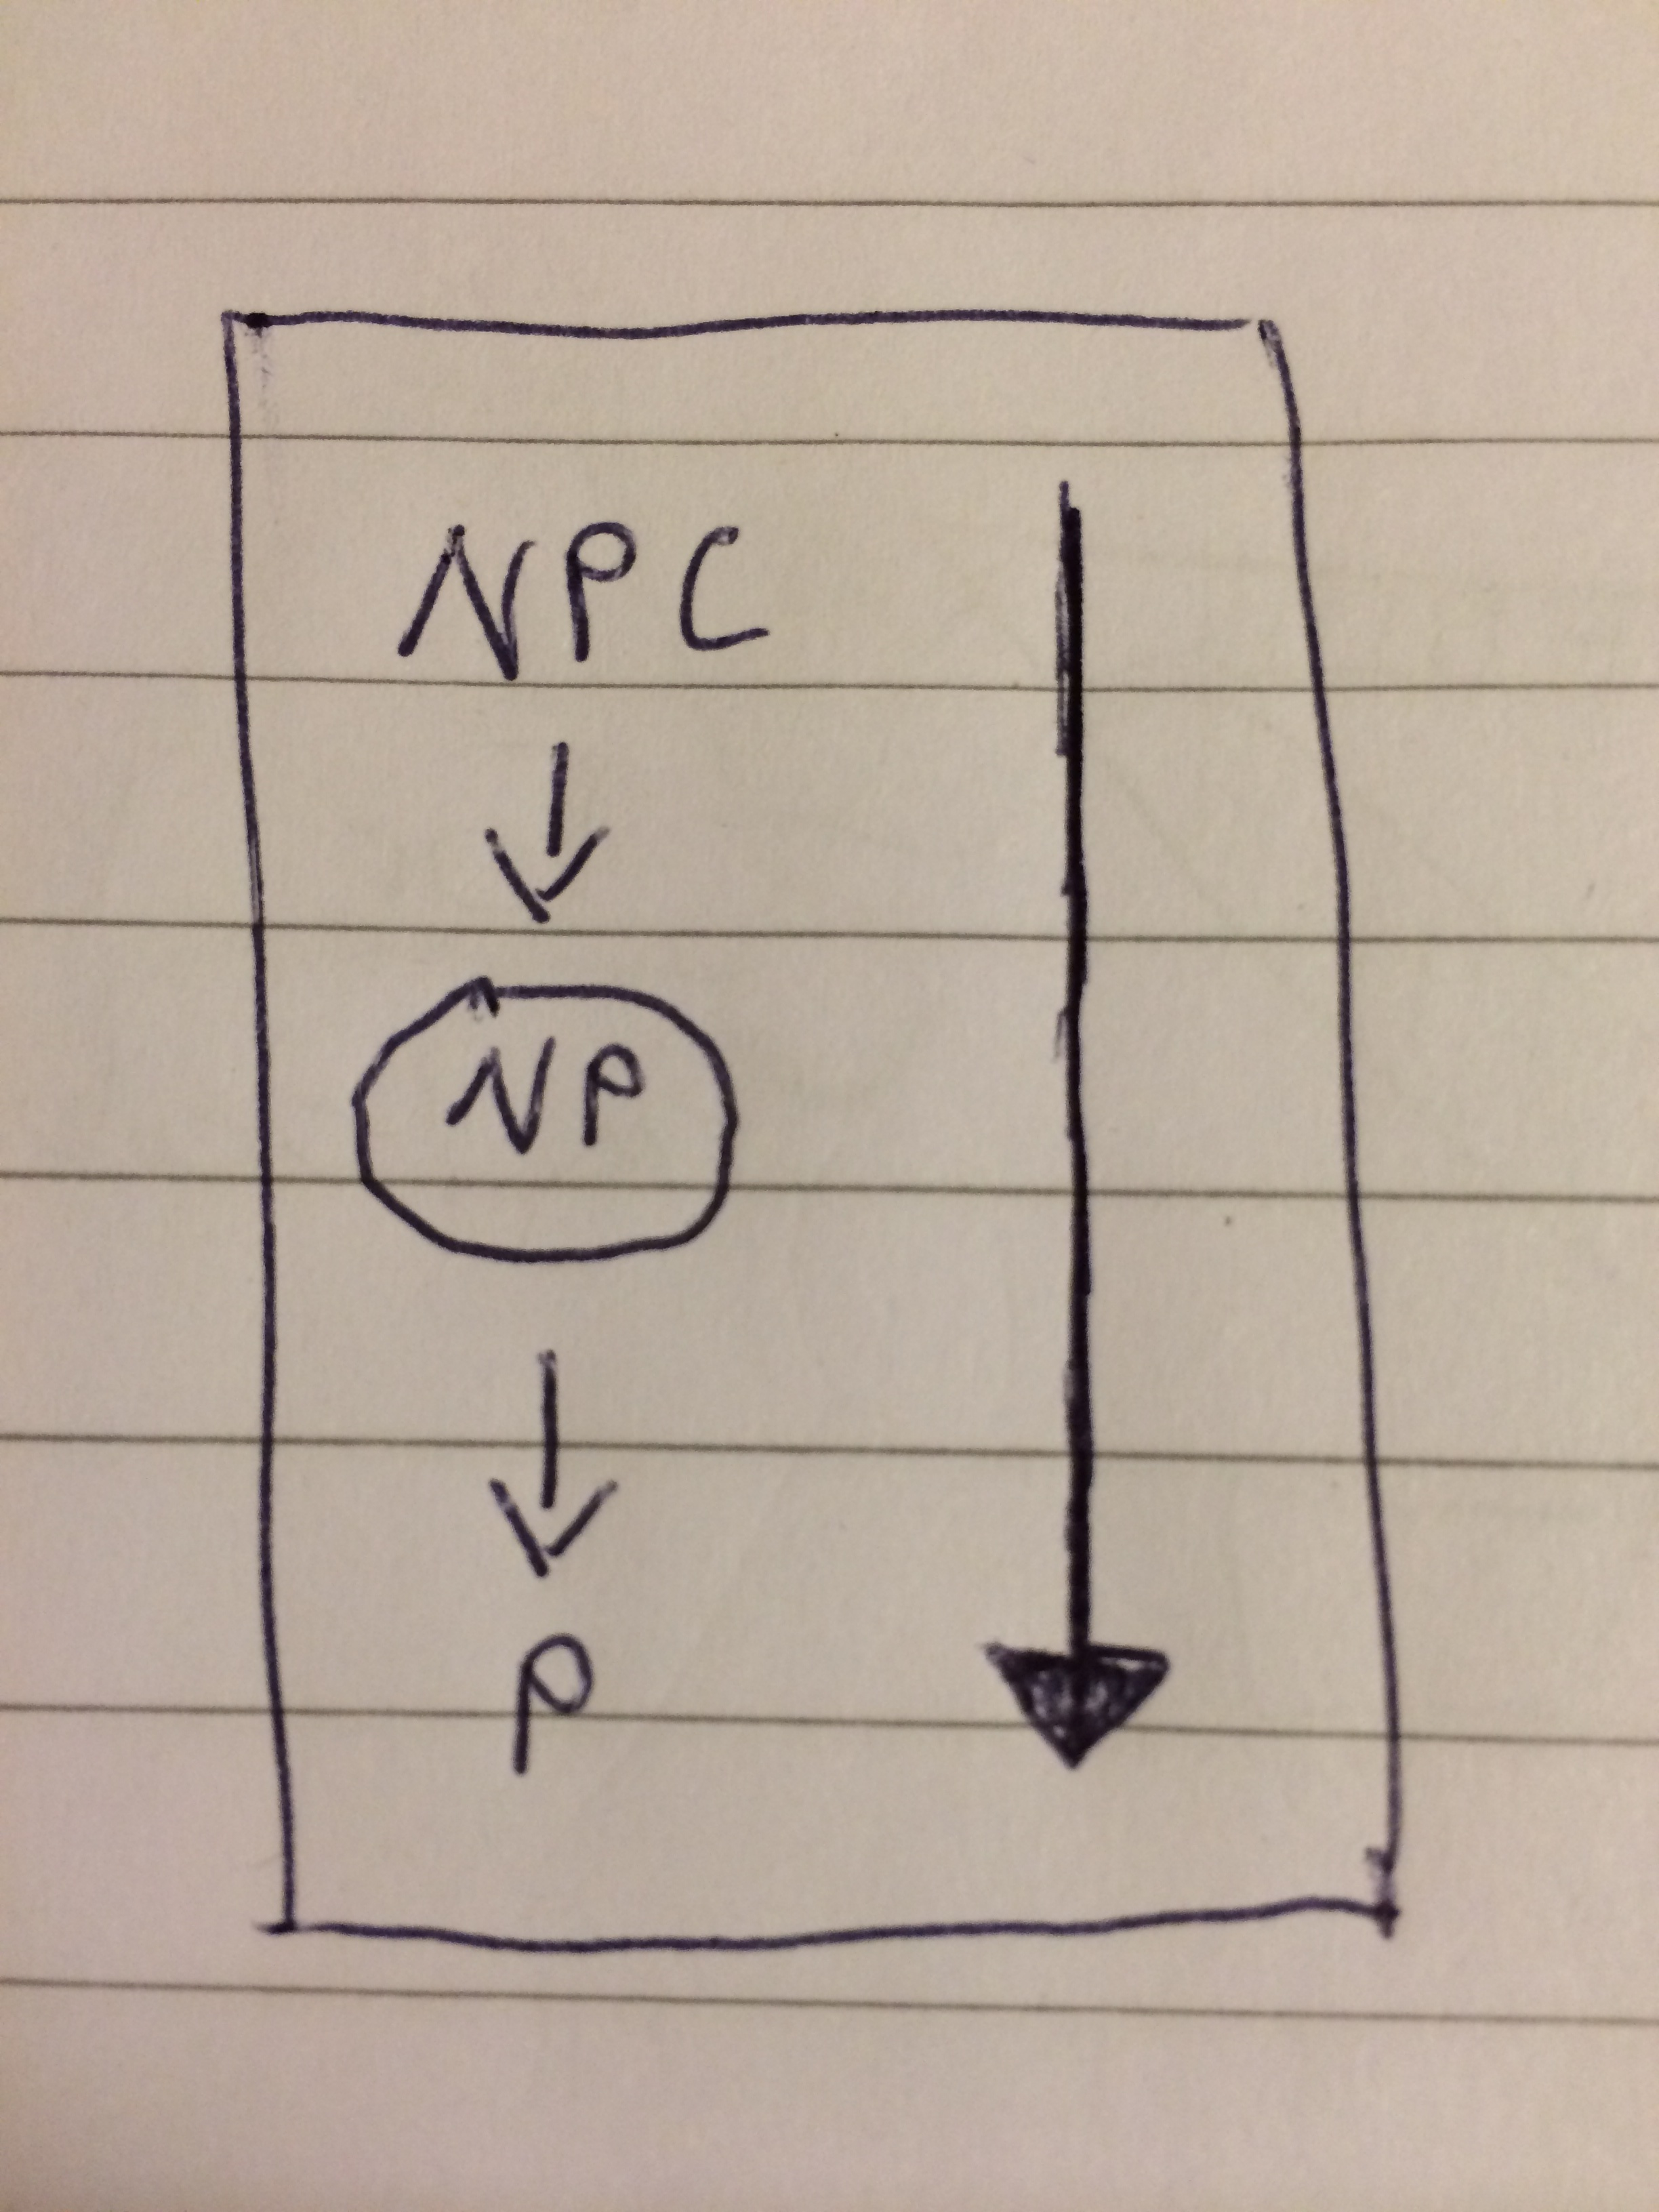
\includegraphics[width=3cm] {cheat.jpg}
        \caption{En tvilsom huskeregel, NB!}
    \end{center}
\end{figure}

\noindent \textbf{Liste/strukturen til NPC-problemer redusert fra CIRCUT-SAT:}

\begin{itemize}
\item CIRCUT-SAT
\item SAT
\item 3-CNF-SAT
	\begin{itemize}
		\item SUBSET-SUM
		\item CLIQUE
		\begin{itemize}
				\item VERTEX-COVER
				\item HAM-CYCLE
				\item TSP (Traveling Salesman Problem)
		\end{itemize}
	\end{itemize}
\end{itemize}

\begin{center}
\begin{figure}[hbt]
    \begin{center}
        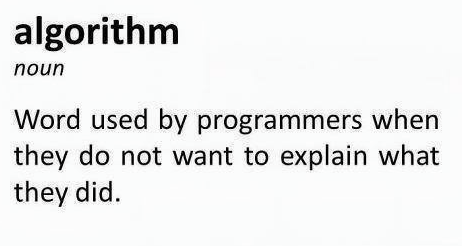
\includegraphics[width=10cm] {algo.png}
        \caption{En avsluttende gave}
    \end{center}
\end{figure}
\end{center}

\section{Pugg disse her for sikkerhetsskyld}

Floyd-Warshall rekurrensen: \\ 

\begin{center}
${D_{ij}^{(k)} = min(${D_{ij}^{(k-1)}, {D_{ik}^{(k-1)} + {D_{kj}^{(k-1)})$ \\ \\
\end{center}

\noindent 0-1 Knapsack-rekurrensen: \\

\begin{center}
$m[i, w] = m[i-1, w]$ if ${w_{i}} > w$ \\ 
$m[i, w] = max(m[i-1], w], m[i-1,w-{w_{i}}] + {v_{i}})$ if ${w_{i}} \leq w$
\end{center}

\end{document}
